\documentclass{article}
\usepackage{tikz}

\title{Circle Graphs}
\author{Alex Katsenelenbogen}

\setlength{\voffset}{-0.75in}

\begin{document}
\begin{center}
      \Large\textbf{Pie Graph}\\
      \large\textit{Prepared by Alex Katsenelenbogen}
   \end{center}
   
   

\begin{center}
\begin{tikzpicture}[thick]
\draw (0,0) circle (4cm);
\draw[very thick,fill=blue!30] (0,0) --  (120:4) arc(120:20:4) -- cycle;
\node (cat) at (70:2.2){\textbf{ferrets}};
\draw[very thick,fill=green!30] (0,0) --  (220:4) arc(220:120:4) -- cycle;
\node (cat) at (180:2.2){\textbf{crows}};
\draw[very thick,fill=yellow!30] (0,0) --  (250:4) arc(250:220:4) -- cycle;
\node (cat) at (233:2.2){\textbf{cats}};
\draw[very thick,fill=red!30] (0,0) --  (380:4) arc(380:250:4) node[pos=0.2] {blah}-- cycle;
\node (cat) at (310:2.2){\textbf{chipmunks}};
\end{tikzpicture}
\end{center}

The above graph shows the breakdown of pet ownership in Rockville. (It does look like folks have \textit{unusual} taste.) 
In any case, The breakdown is as follows:
\begin{itemize}
\item 500 pets were counted
\item Chipmunks make up 180 pets.
\item Crows make up 145 pets.
\item Cats make up 50 pets. 
\item Ferrets make up the rest. 
\end{itemize}
\vspace{1cm}
\noindent
\textbf{\Large{Problems}}
\vspace{0.5cm}
\begin{enumerate}
\item 
For each of pet, calculate the degree measure in both radians and degrees
of the corresponding circle sector.
\item
If the radius of the above pie graph is 4 cm, calculate the area of each sector.
\item
If the radius of the above pie graph is instead 3 cm, calculate the arc length 
for each sector.
\item Verify that for the above questions, the calculated areas and arc lengths
add up to the total area and total circumference respectively.
\end{enumerate}
\end{document}
